\graphicspath{ {imgs/} }
\documentclass[main.tex]{subfiles}
\begin{document}
\chapter{Methods}\label{chap:methods}
The following sections highlight the used methods and give a rough overview about the used tools. First the   A more extensive explanation to the different software packages and computational resources can be found in the appendix.

\section{Software Packages}
Writing a program for solving the task of nodule detection with neural networks 

TensorFlow was chosen since the outset of the research question required a deeper analysis of the neural network at hand. Other possible choices included Keras and Caffe . Keras was discarded for the high level API and potential conflicts later in the analysis. Caffe and TensorFlow would have both seemed well suited, but Tens


\begin{figure}
\begin{center}
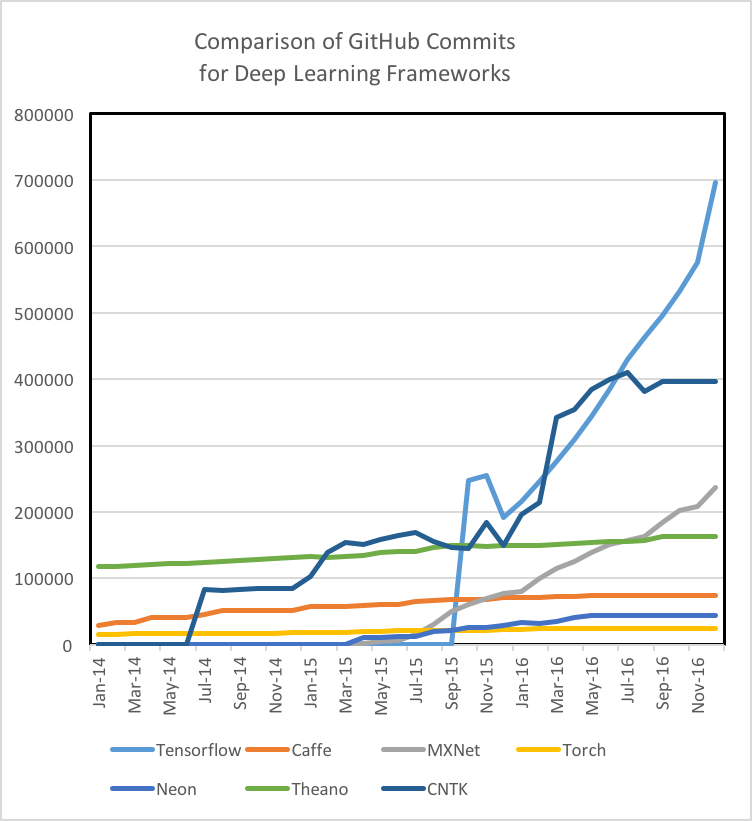
\includegraphics[scale=0.7]{deeplearning_frameworks.png}
\end{center}
\caption{Number of commits for the different deep learning frameworks. This figure is taken from \cite{shapiro2017}}
\label{fig:frameworks}
\end{figure}



- Caffe / Caffe2
- Theano / TensorFlow
- Torch / PyTorch


The whole programming is done in Python 3.6 with the use of conda for managing the installed packages and environments. The Sun Grid Engine of the Institute is used for the execution on the grid \ref{appendix:oge}. For implementing the neural network and measuring it's performance TensorFlow is used. The visualization of the learned filters is done through a combination of tools ranging from matplotlib over GMT ....

\section{Convolutional Neural Network}
In this thesis the main focus was on using a 3d convolutional network. 

Why use this tool? - Convolutional neural networks because of image . 3D because of morphology of the object to be detected, not quite possible to discern from only 2D information, scrolling through the slices.

A convolutional neural network is similar to other artificial neural networks (ANNs) in the sense that it only uses forward connections, has an input and output layer and an arbitrary number of hidden layers in between. The hidden layers in a convolutional network are either convolutional or pooling layers. 

Increasing depth to go from detail features like edges to more complex shapes.

Makes sense to use since the structural information like the neighborhood information can be used


The structure of the neural network resembles closely the one described in \cite{huang2017lung}. 



\section{Training}
The input to the network are the slices that have been the result of the before described preprocessing and are fed to the network in batches. They are augmented by randomly flipping them in x and y plane (examples can be seen in \ref{fig:input}). The augmentation es applied to make the trained network more robust to 

\begin{figure}
\begin{center}
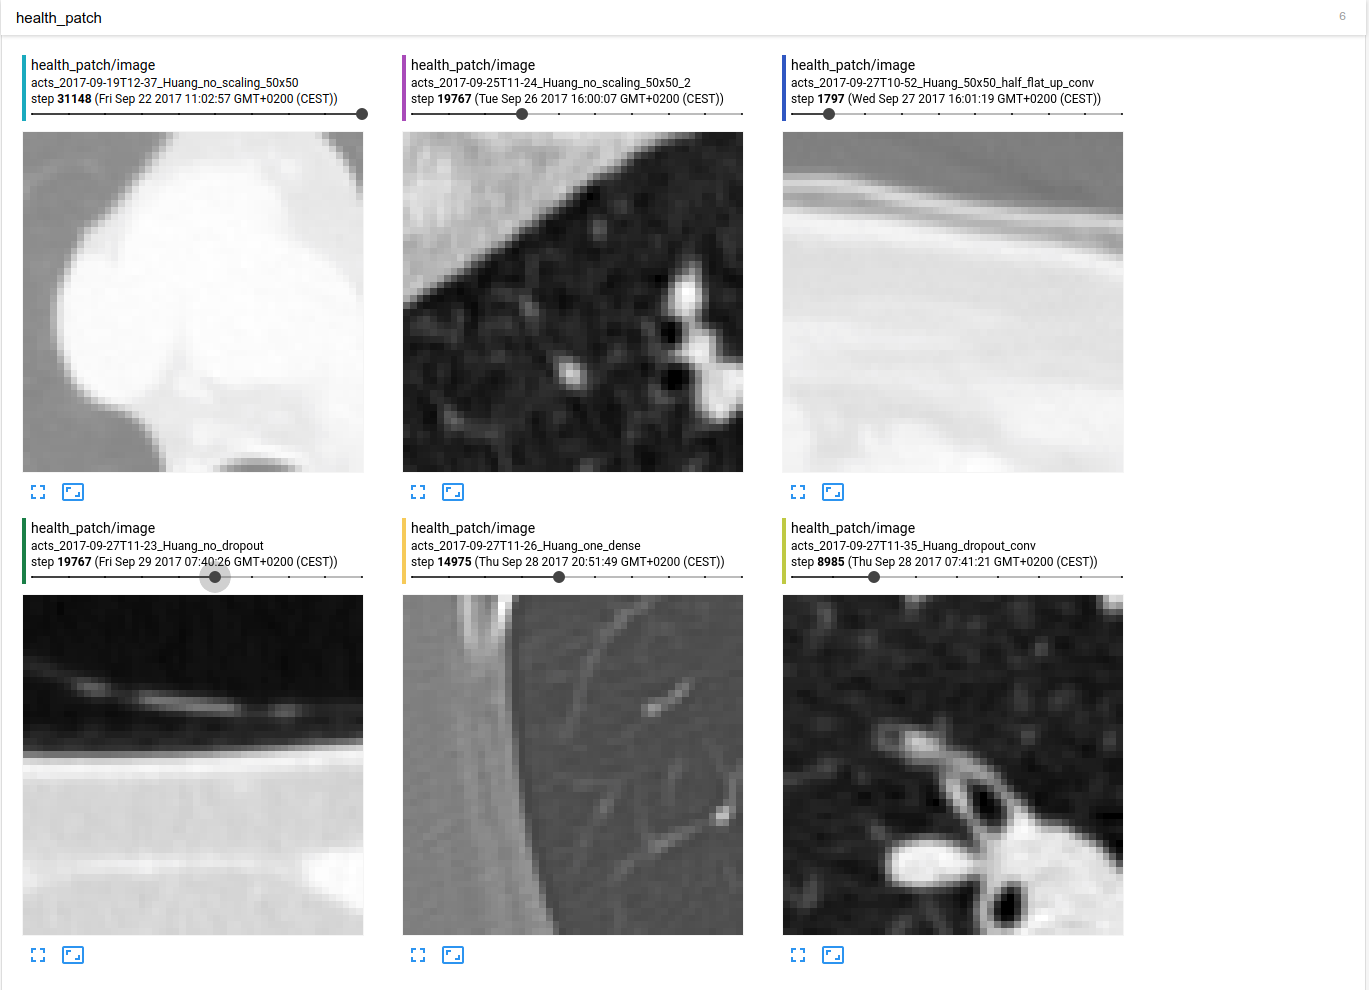
\includegraphics[scale=0.25]{patches-health.png}
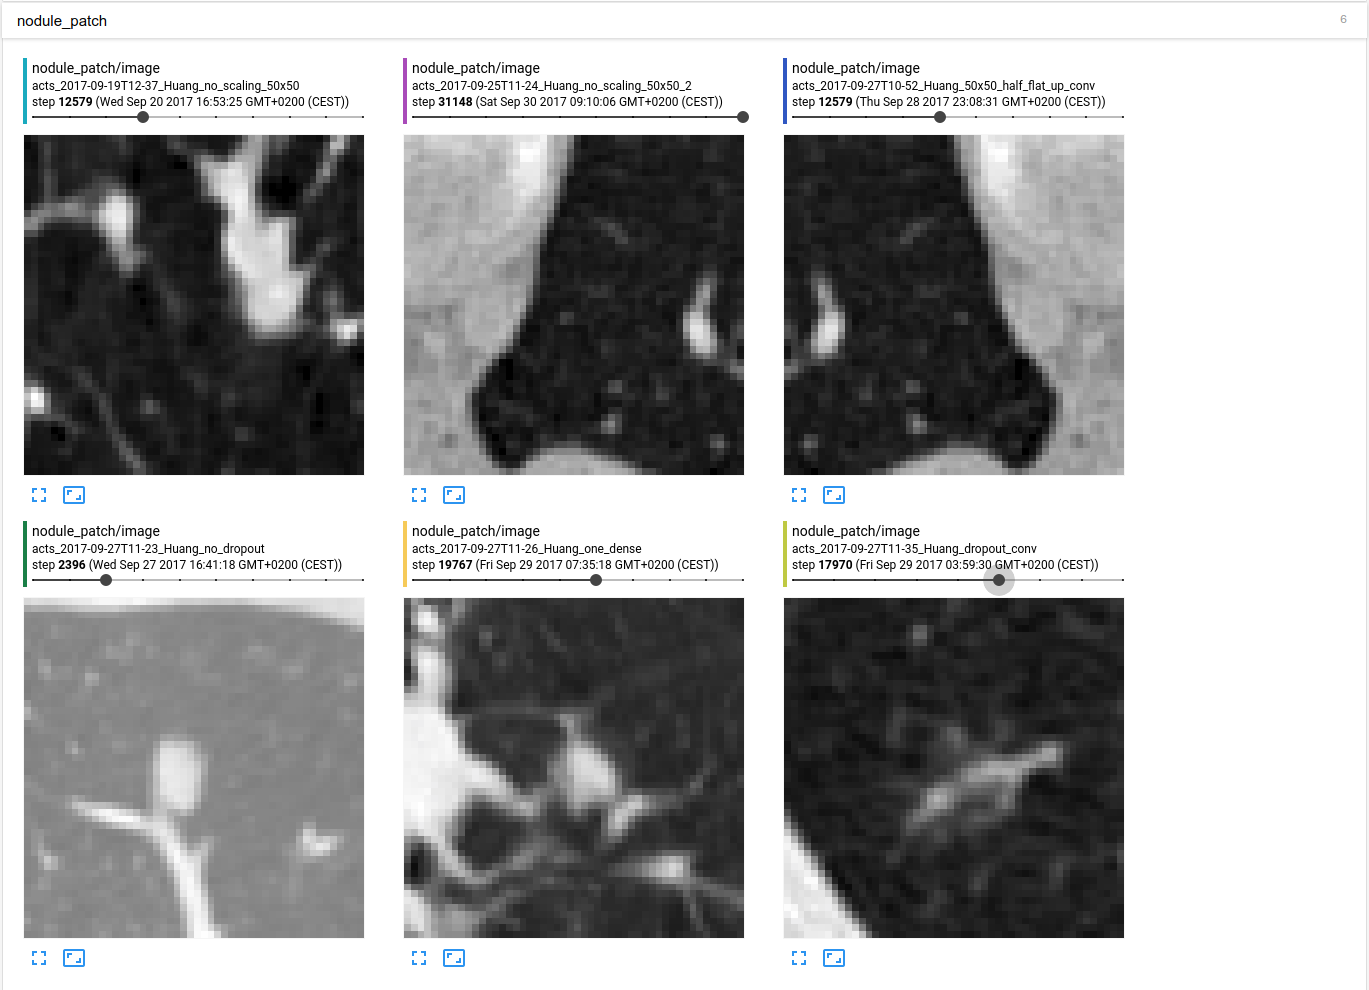
\includegraphics[scale=0.25]{patches-nodule.png}
\end{center}
\caption{Input data for the cases of healthy and nodule patches. The image is taken from Tensorboard and shows in the case of nodules the random permutation of the input data.}
\label{fig:input}
\end{figure}

Why use batchnorm?
Why use dropout?
Compare with and without



\end{document}
